\section{RLPBWT con matching statistics}
\label{secrlpbwtms}
Le precedenti versioni della \textit{RLPBWT}, come anticipato, hanno permesso di
poter ideare una variante \textit{run-length encoded} della \textit{PBWT}.
In realtà anche in questo caso c'è stata una fase transitoria di sviluppo,
avendo due varianti della struttura, che verranno introdotte a breve.\\
Il fine era quello di ottenere quanto visto per la \textbf{RLBWT} anche per la
variante posizionale, ovvero i concetti di:
\begin{itemize}
  \item \textit{matching statistics}
  \item \textit{threshold}
  \item \textit{LCE query}
\end{itemize}
A tal fine, come per la \textit{RLBWT}, si necessita di \textit{random access}
al pannello. A causa di questo si sono avute due varianti in fase di sviluppo:
\begin{itemize}
  \item una prima, ancora in ottica di ``studio introduttivo'', dove il pannello
  viene memorizzato come \textit{vettore di bitvector classici}
  \item una seconda, definitiva, dove il pannello è memorizzato come
  \textit{SLP}, nelle modalità introdotte nella sottosezione \ref{subslp}
\end{itemize}
Queste versioni, a loro volta, hanno permesso, in primis, l'ideazione di un
algoritmo che sfruttasse l'idea delle threshold, come visto per la \textit{BWT}
classica con \textit{MONI} \cite{moni}, e poi, per quella basata
sull'\textit{SLP}, di uno basato sulle \textit{LCE query}, come per
\textit{PHONI} \cite{phoni}. Quest'ultima, con l'aggiunta della
\textit{struttura per la funzione $\varphi$}, sarà l'implementazione definitiva,
per questa tesi, della \textit{RLPBWT}.\\
Avendo in memoria il pannello si può quindi fare a meno dell'array \textit{LCP}
della colonna $k$-esima, avendo quindi che, per ogni colonna $k$, si ha in
memoria:
\begin{itemize}
  \item un booleano $start^k$ per specificare se la colonna presenta la prima
  run costruita su simboli $\sigma =0$
  \item un bitvector sparso $h_k$ per indicare l'inizio delle run
  \item il valore $c[k]$ per sapere quanti simboli $\sigma=0$ si hanno nella
  colonna 
  \item i valori $u_k$ e $v_k$ per il mapping
  \item i cosiddetti \textbf{prefix array samples}, ovvero i valori del
  \textbf{prefix array} di inizio e fine di ogni run. Si noti quindi che, anche
  in questo caso, si ha un'informazione in memoria proporzionale al numero di
  run $r$ 
\end{itemize}
In pratica si hanno in memoria le stesse informazioni della \textit{RLPBWT con
  bitvector} al più di $l_k$, ovvero l'\textit{array LCP} della colonna
$k$-esima, e dei \textit{prefix array samples}. 
\subsection{Matching statistics per la RLPBWT}
La definizione formale per il concetto di \textbf{matching statistics}, nonché
il calcolo dell'array stesso, vista per
la \textit{RLBWT} deve essere ovviamente riadattata allo studio di match tra un
aplotipo e un pannello di aplotipi.
\begin{definizione}
  Dato un pannello $X$, di dimensioni $M\times N$, con $M$ individui e $N$ siti,
  e un aplotipo esterno/pattern $z$, tale che $|z|=N$, si definisce matching
  statistics di $z$ su $X$ un array $MS$ di coppie $(row,len)$, di lunghezza
  $N$, tale che (avendo che $x_i$ indica l'$i$-esima riga del pannello $X$): 
  \begin{itemize}
    \item $x_{MS[i].row}[i-MS[i].len+1,i]=z[i-MS[i].len+1,i]$, ovvero si ha che
    l'aplotipo query ha un match, terminante in colonna $i$, con la riga
    $MS[i].row$  
    \item $z[i-MS[i].len,i]$ non è un suffisso terminante in colonna $i$ di un
    qualsiasi sottoinsieme di righe di $X$. In altri termini il match non deve
    essere ulteriormente estendibile a sinistra
  \end{itemize}
\end{definizione}
Inoltre, analogamente al caso della variante classica, si ha il seguente lemma.
\begin{lemma}
  Dato un pannello $X$, di dimensioni $M\times N$, con $M$ individui e $N$
  siti, un aplotipo esterno/pattern $z$, tale che $|z|=N$, e il corrispondente
  array di matching statistics $MS$ si ha che:
  \[z[i-l+1,i]\]
  è uno \textbf{SMEM} di lunghezza $l$ in con la riga $MS[i].row$ del pannello
  $X$ sse: 
  \[MS[i].len=l\land(i=N-1\lor MS[i].len\geq MS[i+1].len)\]
\end{lemma}
\textit{Si vedrà in sezione \ref{secphi} come calcolare, a partire da tali
  \emph{SMEM}, tutte le righe del panello per le quali si ha lo stesso
  \textup{SMEM}}.\\
Il calcolo dell'array $MS$ di $z$ rispetto al pannello $X$ si basa su due fasi:
\begin{enumerate}
  \item la fase di \textbf{extension}
  \item la fase di \textbf{bootstrap}
\end{enumerate}
Si assuma di avere due indici $i$ e $j$, $0\leq i\leq j\leq N$, tali per cui
$z[i,j]$ è un suffisso di uno tra $x_1[1,j]$, \ldots, $x_M[1,j]$. \\
La \textbf{fase di extension} estende il match di $z[i,j]$ a $z[i,j+1]$ sse:
\begin{itemize}
  \item $j<M$
  \item $z[i,j+1]$ è un suffisso di uno tra $x_1[1,j+1]$, $\ldots$, $x_M[1,j+1]$
\end{itemize}
D'altro canto la \textbf{fase di bootstrap} cerca il più piccolo indice $i'$,
avendo $i\leq i'\leq j$, tale per cui $z[i',j]$ è un suffisso di uno tra
$x_1[1,j+1]$, $\ldots$, $x_M[1,j+1]$.\\
Si ha quindi il computo di ogni valore $MS[i]$, $\forall i\in[0,N)$, dell'array
delle \textit{matching statistics}:
\begin{itemize}
  \item si assume inizialmente che $MS[0].len=0$
  \item si applica la \textit{fase di bootstrap} per cercare il minimo indice
  $i'$, avendo $i\leq i'$, tale che $z[i',i'+MS[i].len]$ è un suffisso di uno
  tra $x_1[1,i'+MS[i].len],$ \ldots$, x_M[1,i'+MS[i].len]$. Inoltre, per
  minimalità di $i'$ si ha che, $\forall i<j<i'$, $MS[j].len=MS[j-1].len+1$
  \item a questo punto si itera la \textit{fase di estensione} per trovare il
  più lungo prefisso $z[i',k]$ che è anche un suffisso di uno tra $x_1[1,k]$,
  $\ldots$, $x_M[1,k]$, avendo che $MS[i'].len=k-i'+1$
  \item avendo che $i'>i$ si può procedere induttivamente al calcolo dell'array
  $MS$ 
\end{itemize}
\textbf{PARTE PRESA DAL PAPER: RIVEDERE PROFONDAMENTE}.\\
In altri termini, più ``pratici'', il calcolo dell'array $MS$ avviene nel
seguente modo:
\begin{itemize}
  \item si parte da una riga arbitraria $i$ della prima colonna
  \item se $x_i[0]=z[0]$ si procede salvando $MS[0].row=i$
  \item qualora si abbia $x_i[0]\neq z[0]$ si seleziona o l'ultima riga della
  run precedente o la prima riga della run successiva a quella a cui appartiene
  la riga $i$. Tale riga, $j$, verrà salvata in $MS$, avendo $MS[0].row=j$
  \item a questo punto si effettua il mapping verso la colonna successiva, $k$,
  e, a seconda di avere un match con $z[k]$ si procede come nei casi visti sopra
\end{itemize}
Si noti che non si è parlato di come calcolare i vari $MS[i].len$, questo in
quanto si hanno due soluzioni (che verranno poi approfondite), che riprendono
appunto \textit{MONI} e \textit{PHONI} per la \textit{RLBWT};
\begin{enumerate}
  \item si possono usare le threshold per capire che nuova riga selezionare in
  caso di mismatch. In tal caso i vari $MS[i].len$ devono essere calcolati dopo
  il calcolo di $MS[i].row$ tramite \textit{random access} al panel
  \item si possono usare le \textit{LCE query} per capire che nuova riga
  selezionare in caso di mismatch e in tal caso il calcolo delle $MS[i].len$
  avviene in contemporanea 
\end{enumerate}
Prima di procedere con i dettagli dei due metodi è bene proporre un veloce
esempio di array $MS$.
\begin{esempio}
  \label{es:ms}
  Si riprenda nuovamente l'esempio \ref{es:algo5}, con un pannello e i match con
  la query $z$:
  \begin{figure}[H]
    \centering
    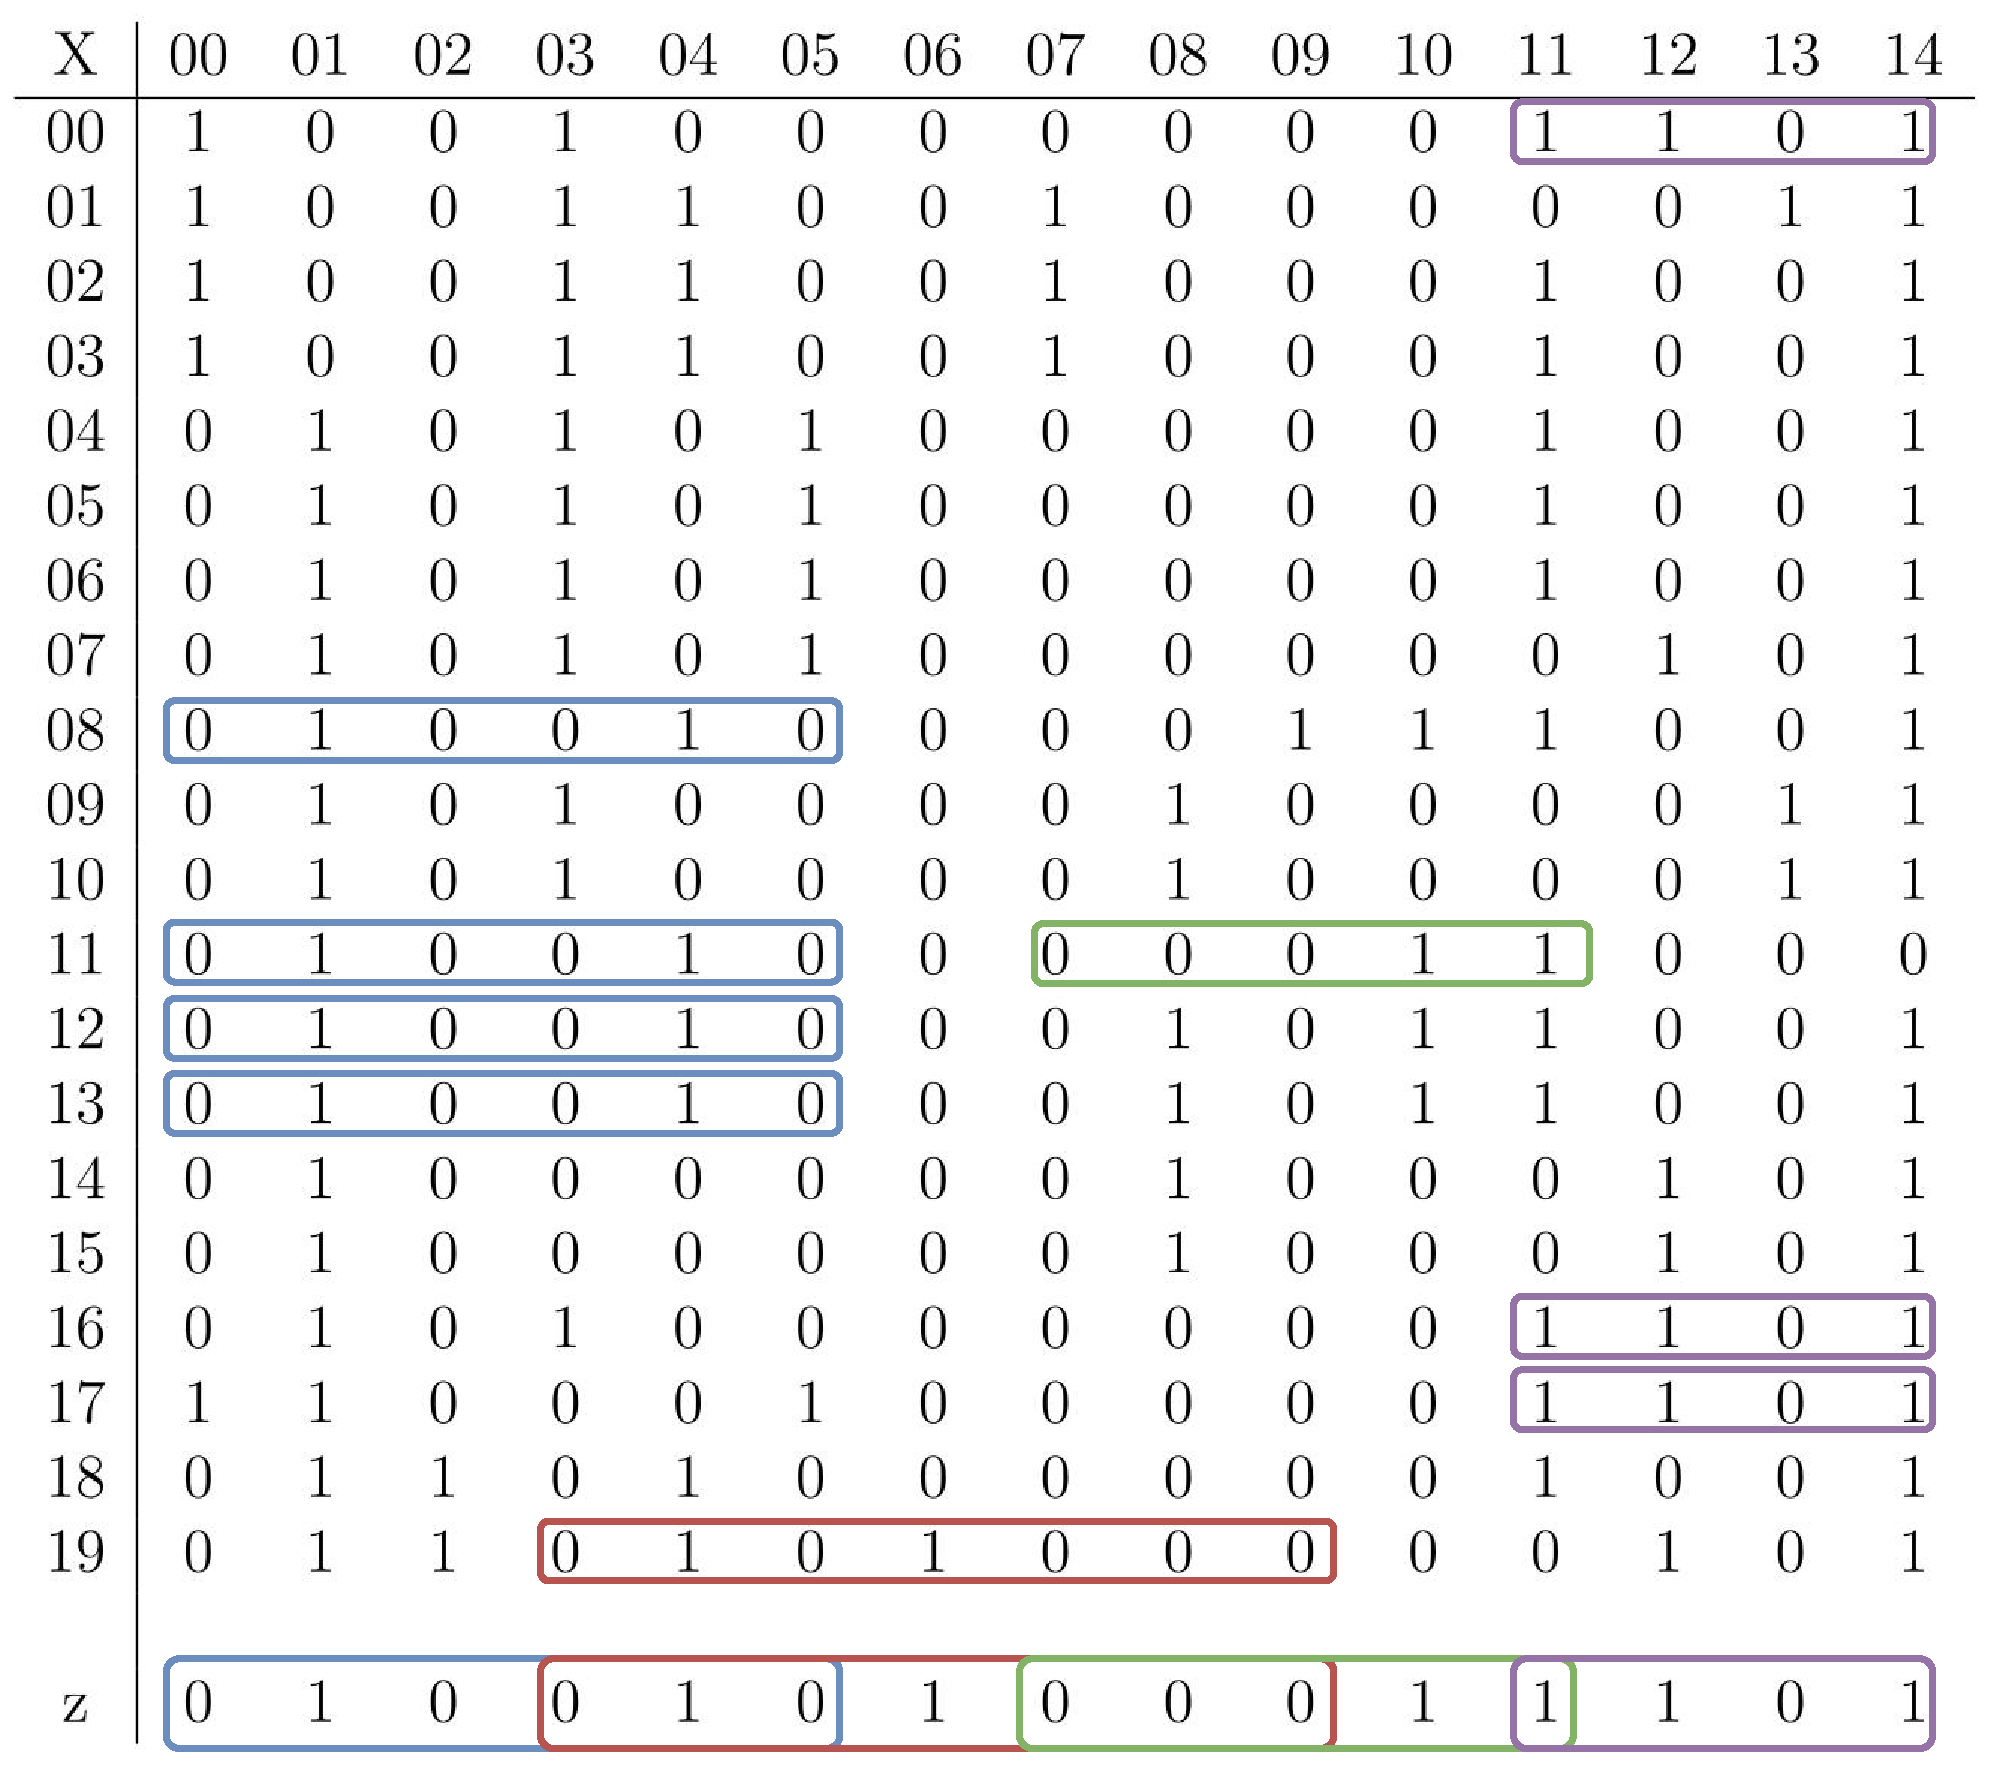
\includegraphics[scale = 0.365]{img/pbwtmatch.pdf}
  \end{figure}
  In tal caso l'array $MS$ sarebbe, avendo scelto come riga iniziale la 19:
  \begin{table}[H]
    \footnotesize{}
    \centering
    \begin{tabular}{c|ccccccccccccccc}
      $k$ & 00 & 01 & 02 & 03 & 04 &  {\color{nordgreen}05} & 06 & 07 & 08
      &  {\color{nordgreen}09} & 10 &  {\color{nordgreen}11} & 12 & 13
      &  {\color{nordgreen}14} \\
      \hline
      \hline
      $z$ & 0 & 1 & 0 & 0 & 1 &  {\color{nordgreen}0} & 1 & 0 & 0
      &  {\color{nordgreen}0} & 1 &  {\color{nordgreen}1} & 1 & 0
      &  {\color{nordgreen}1} \\
      \hline
      $row$ & 19 & 19 & 16 & 15 & 13 &  {\color{nordgreen}13} & 19 & 19 & 19
      &  {\color{nordgreen}19} & 11 &  {\color{nordgreen}11} & 17 & 17
      &  {\color{nordgreen}17} \\
      $len$ & 1 & 2 & 3 & 4 & 5 & {\color{nordgreen}6} & 4 & 5 & 6
      & {\color{nordgreen}7} & 4 & {\color{nordgreen}5} & 2 & 3
      & {\color{nordgreen}4}\\
    \end{tabular}
  \end{table}
  Dove si possono riconoscere i vari \textit{SMEM}, la cui colonna di fine è
  segnalata in verde, secondo la definizione data
  sopra (anche in questo caso i dettagli del calcolo
  verranno esplicitati successivamente). 
\end{esempio}
\subsection{Threshold per la RLPBWT}
Come anticipato una prima strategia per la scelta di una nuova riga $j$, qualora
la precedente riga $i$ comporti un mismatch in colonna $k$ con l'aplotipo query,
avendo $x_i[k]\neq z[k]$ è l'utilizzo delle \textbf{threshold}.
\begin{definizione}
  Data la colonna $k$-esima della \textbf{matrice PBWT}, $y^k$, memorizzata
  tramite compressione \textbf{run-length} e data la run $j$-esima, indicizzata
  da $i$ a $i'$, si definisce \textbf{threshold} come l'indice del minimo valore
  \textit{LCP}, che ricordiamo essere calcolato sull'ordinamento inverso,
  compreso negli indici della run, compreso l'eventuale 
  $LCP_k[i'+1]$, qualora $i'\neq M-1$. Si noti che quest'ultimo valore, se
  esistente, deve essere considerato in quanto per il suo calcolo, come
  specificato nei preliminari alla sezione \ref{secpbwt}, si prende in
  considerazione $y^k_{i'}$ e $y^k_{i'+1}$.
\end{definizione}
Con tale informazione, unita ai \textit{prefix array sample}, si può quindi
ottenere un comportamento analogo a quanto si ottiene con l'\textbf{R-index} per
la \textit{RLBWT}.\\
Sia infatti data $t$ la posizione della \textit{threshold} nella run corrente,
in colonna $k$, e
si supponga che tale run, con testa all'indice $h$, non sia associata al simbolo
desiderato, ovvero $z[k]$. Si supponga che, con il mapping, si sia arrivati
all'indice $i$ della colonna $k$. Si supponga inoltre che la run successiva
abbia testa in indice $e$. Si hanno due casi possibili, denotando con
$LCS(x,y)$ il \textit{longest common suffix} tra le stringhe $X$ e $Y$ e con
$a_k$ il \textit{prefix array} in colonna $K$:
\begin{enumerate}
  \item $i<t$ allora, per definizione di \textit{threshold}:
  \[LCS(z[0,k], x_{a_{k}[h-1]}[0,k])\geq LCS(z[0,k], x_{a_{k}[e]}[0,k])\]
  Quindi si ha che $MS[k].row=a_{k}[h-1]$ e il mapping potrà proseguire
  dall'indice $h-1$
  \item  $i\geq t$ allora, per definizione di \textit{threshold}:
  \[LCS(z[0,k], x_{a_{k}[h-1]}[0,k])\leq LCS(z[0,k], x_{a_{k}[e]}[0,k])\]
  Quindi si ha che $MS[k].row=a_{k}[e]$ e il mapping potrà proseguire
  dall'indice $e$
\end{enumerate}
Qualora una colonna presenti solo simboli $\sigma\neq z[k]$, per convenzione, si
imposta che $MS[k].row = M$ e si ricomincia, in colonna $k+1$, dall'ultima
posizione, indicizzata nel pannello originale dal valore finale del
\textit{prefix array sample} dell'ultima run.\\
In termini implementativi anche le posizioni delle \textit{threshold} vengono
memorizzate tramite un \textit{bitvector sparso} per ogni colonna $k$, avendo
che, qualora il minimo \textit{LCP} si ritrovi nell'indice della testa della run
successiva, la posizione della threshold verrà comunque memorizzata all'indice
della coda della run corrente. Purtroppo questa è una situazione di ambiguità,
avendo che, seguendo la definizione sopra, avendo la \textit{threshold} a fine
run, bisognerebbe scegliere la testa della run successiva, qualora l'indice $i$
si trovi esattamente a fine run. Invece, qualora la
\textit{threshold} sia a fine run a causa del fatto che il minimo \textit{LCP}
si trovi nella testa della run successiva, bisogna scegliere la coda della run
precedente. L'unico modo per disambiguare è quindi effettuare \textit{random
  access} al pannello per vedere quale sia la
soluzione migliore, ovvero quale tra la coda della run precedente e la testa
della run successiva siano relative alla riga del pannello originale con un
suffisso comune alla query più lungo.\\
Purtroppo non è possibile salvare la threshold direttamente nella testa della
run successiva in quanto questa potrebbe essere anche la posizione della
threshold della run successiva e avere due threshold sovrapposte impedirebbe di
capire a quale run appartiene una certa threshold, tramite la funzione
\textit{rank}. \\
Tale bitvector deve essere quindi aggiunto alle informazioni memorizzate per
ogni singola colonna. Lo pseudocodice per la costruzione di una colonna con
anche il bitvector per le \textit{threshold} è consultabile all'algoritmo
\ref{algo:cosbv}. 
\begin{esempio}
  \label{es:thr}
  Si vede quindi un esempio di funzionamento delle threshold.\\
  Si prenda pannello visto all'esempio \ref{es:pbwt1} e si effettui la
  permutazione secondo $a_2$:
  \begin{table}[H]
    \centering
    \footnotesize
    \begin{tabular}{c|cc|c|cccccccccccc}
      X & 00 & 01 & 02 & 03 & 04 & 05 & 06 & 07 & 08 & 09 & 10 & 11 & 12 & 13
      & 14 \\
      \hline
      00 & 1 & 0 & 0 & 1 & 0 & 0 & 0 & 0 & 0 & 0 & 0 & 1 & 1 & 0 & 1 \\
      01 & 1 & 0 & 0 & 1 & 1 & 0 & 0 & 1 & 0 & 0 & 0 & 0 & 0 & 1 & 1 \\
      02 & 1 & 0 & 0 & 1 & 1 & 0 & 0 & 1 & 0 & 0 & 0 & 1 & 0 & 0 & 1 \\
      03 & 1 & 0 & 0 & 1 & 1 & 0 & 0 & 1 & 0 & 0 & 0 & 1 & 0 & 0 & 1 \\
      04 & 0 & 1 & 0 & 1 & 0 & 1 & 0 & 0 & 0 & 0 & 0 & 1 & 0 & 0 & 1 \\
      05 & 0 & 1 & 0 & 1 & 0 & 1 & 0 & 0 & 0 & 0 & 0 & 1 & 0 & 0 & 1 \\
      06 & 0 & 1 & 0 & 1 & 0 & 1 & 0 & 0 & 0 & 0 & 0 & 1 & 0 & 0 & 1 \\
      07 & 0 & 1 & 0 & 1 & 0 & 1 & 0 & 0 & 0 & 0 & 0 & 0 & 1 & 0 & 1 \\
      08 & 0 & 1 & 0 & 0 & 1 & 0 & 0 & 0 & 0 & 1 & 1 & 1 & 0 & 0 & 1 \\
      09 & 0 & 1 & 0 & 1 & 0 & 0 & 0 & 0 & 1 & 0 & 0 & 0 & 0 & 1 & 1 \\
      10 & 0 & 1 & 0 & 1 & 0 & 0 & 0 & 0 & 1 & 0 & 0 & 0 & 0 & 1 & 1 \\
      11 & 0 & 1 & 0 & 0 & 1 & 0 & 0 & 0 & 0 & 0 & 1 & 1 & 0 & 0 & 0 \\
      12 & 0 & 1 & 0 & 0 & 1 & 0 & 0 & 0 & 1 & 0 & 1 & 1 & 0 & 0 & 1 \\
      13 & 0 & 1 & 0 & 0 & 1 & 0 & 0 & 0 & 1 & 0 & 1 & 1 & 0 & 0 & 1 \\
      14 & 0 & 1 & 0 & 0 & 0 & 0 & 0 & 0 & 1 & 0 & 0 & 0 & 1 & 0 & 1 \\
      15 & 0 & 1 & 0 & 0 & 0 & 0 & 0 & 0 & 1 & 0 & 0 & 0 & 1 & 0 & 1 \\
      16 & 0 & 1 & 0 & 1 & 0 & 0 & 0 & 0 & 0 & 0 & 0 & 1 & 1 & 0 & 1 \\
      17 & 0 & 1 & 1 & 0 & 1 & 0 & 0 & 0 & 0 & 0 & 0 & 1 & 0 & 0 & 1 \\
      18 & 0 & 1 & 1 & 0 & 1 & 0 & 1 & 0 & 0 & 0 & 0 & 0 & 1 & 0 & 1 \\
      19 & 1 & 1 & 0 & 0 & 0 & 1 & 0 & 0 & 0 & 0 & 0 & 1 & 1 & 0 & 1 \\
    \end{tabular}
  \end{table}
  Si prenda la seconda run, di simboli $\sigma=1$, indicizzata tra 17 e 18. \\
  Si supponga che, tramite il mapping, si sia arrivati alla riga 17 ma che si
  abbia $z[2]=0$. la scelta è quindi tra la coda della run precedente, avendo
  che $a_2[16]=16$ o la testa della run successiva, avendo che $a_2[19]=17$. Si
  può notare come il minimo \textit{LCP} si trovi, per la 
  run, all'indice 18 (a causa del fatto che il minimo \textit{LCP} è all'indice
  19, quello della testa della run successiva). Si può quindi proseguire o con
  la riga. Questo significa che il suffisso comune più lungo con la query si ha
  con la riga 16 del pannello, per definizione di threshold, avendo che questa
  sarà memorizzata nell'array $MS$:
  \[MS[2].row=16\]
  Successivamente, tramite \textit{random access} al testo, confrontando la riga
  $x_{16}$ e la query $z$, fino alla colonna $k=2$, si potrà calcolare che
  $MS[2].len=3$. 
\end{esempio}
\textbf{SISTEMARE ESEMPIO}\\
Una volta computato tutti i valori $MS[i].row$ per calcolare i vari $MS[i].len$
si scorre da sinistra a destra calcolando la lunghezza del match facendo random
access al pannello e confrontando la query $z$ con la riga $MS[i].row$. Si
assuma infatti di aver calcolato $MS[i-1].len$ e di voler calcolare $MS[i].len$.
Si hanno tre casi possibili:
\begin{enumerate}
  \item $MS[i].row=M$ e in tal caso, avendo segnalata l'inesistenza di alcun
  match, si ha che $MS[i].len=0$
  \item $MS[i].row=MS[i-1].row$, avendo $i\neq 0$ e $MS[i-1].len\neq 0$, allora
  si sta seguendo la stessa riga che si seguiva in colonna $i-1$ e quindi,
  banalmente, $MS[i].len=MS[i-1].len+1$
  \item in qualsiasi altro caso bisogna confrontare, a partire dalla colonna
  $i$, la query 
  $z$ con la riga $MS[i].row$ del pannello da destra a sinistra, fino a che non
  si trova un mismatch, calcolando la lunghezza $l$ del suffisso comune tra esse
  e memorizzando tale valore: $MS[i].len=l$
\end{enumerate}
In fase di costruzione delle lunghezze è possibile anche riportare gli
\textit{SMEM}, terminanti in colonna $i$, qualora:
\begin{itemize}
  \item $MS[i].len\geq MS[i+1].len \land MS[i].len\neq 0$
  \item si è arrivati a fine array, avendo $i=N-1\land MS[i].len\neq 0$
\end{itemize}
Come si può verificare nell'esempio \ref{es:ms}.\\
L'algoritmo per il match tramite \textit{threshold} è visualizzabile
all'algoritmo \ref{algo:matchthr}.
\textbf{CAPIRE SE DESCRIVERE ALGORITMO}
\subsection{LCE query per la RLPBWT}
La memorizzazione di un \textit{bitvector sparso} atto a rappresentare le
posizioni delle threshold ha però un costo in memoria. Inoltre, per ora, si è
parlato di tenere in memoria il pannello sotto forma di vettore di
\textit{bitvector} e anche questo ha un costo non indifferente in termini di
spazio necessario.\\
Per arrivare all'implementazione conclusiva della \textit{RLPBWT} si è quindi
optato per la memorizzazione del pannello sotto forma di \textit{SLP}, struttura
che, come anticipato, permette anche di eseguire efficientemente le \textit{LCE
  query}.
\begin{definizione}
  Dato un pannello $X$, $M\times N$, e due righe $x_i$ e $x_j$ tali che $0\leq
  i <m$ e $0\leq j <M$, con $i\neq j$, si definisce \textbf{LCE query} il
  suffisso comune (o il prefisso se considerato l'ordine inverso) più lungo tra
  le due righe. Per comodità nella sezione si 
  definisce la funzione: 
  \[LCE_k(x_i,x_j)=l\]
  dove $l$ è la lunghezza del suffisso comune più lungo tra le due stringhe
  terminante in colonna $k-1$.
\end{definizione}
\subsubsection{Compressione del panel}
Bisogna quindi capire in primis come costruire l'\textit{SLP}. In primis, le
librerie per la costruzione di tale struttura assumono un input
``monodimensionale'', ovvero una singola sequenze lineare. Inoltre, anche per
permettere la costruzione efficiente della \textit{PBWT}, e conseguentemente
della \textit{RLPBWT}, il pannello in input risulta essere trasposto, avendo che
le righe nel file in input rappresentano i siti e non gli individui. Bisogna
quindi in primis trasporre tale pannello. Per procedere ulteriormente bisogna
però ricordare che sull'\textit{SLP} si avrà 
necessità di effettuare \textit{LCE query} che però, si anticipa, nel nostro
pannello, devono essere fatte tra due righe da destra a sinistra (a differenza
di quanto visto nel caso standard dove si confrontavano prefissi comuni). Per
rendere possibile questa operazione quindi il pannello deve essere sia 
salvato come un'unica riga, per ottenerne l'\textit{SLP}, che ``da destra a
sinistra'', per permettere le \textit{LCE query}. Si procede quindi concatenando
ogni riga, selezionandole consecutivamente e leggendone i singoli elementi da
destra a sinistra.
\begin{esempio}
  Si vede quindi un breve esempio.\\
  Si assuma di avere il seguente pannello nel file in input.
  \[
    X=\left[
      \begin{matrix}
        0 & 0 & 1 & 0 & 0\\
        1 & 1 & 1 & 0 & 1\\
        0 & 1 & 1 & 1 & 1\\
        0 & 0 & 0 & 1 & 0
      \end{matrix}
    \right]
  \]
  Dove però come detto le righe sono i siti e le colonne i sample. Per ottenere
  l'\textit{SLP} biosgna quindi, in primis, trasporre la matrice:
  \[
    X^T=\left[
      \begin{matrix}
        0 & 1 & 0 & 0\\
        0 & 1 & 1 & 0\\
        1 & 1 & 1 & 0\\
        0 & 0 & 1 & 1\\
        0 & 1 & 1 & 0
      \end{matrix}
    \right]
  \]
  A questo punto bisogna considerare l'ordine in cui si vorranno effettuare le
  \textit{LCE query}.
  Ad esempio, prendendo la seconda e la terza riga, facendo partire il confronto
  dall'ultima colonna, avremmo una \textit{LCE
    query} lunga 3, terminante nella prima colonna esclusa:
  \begin{figure}[H]
    \centering
    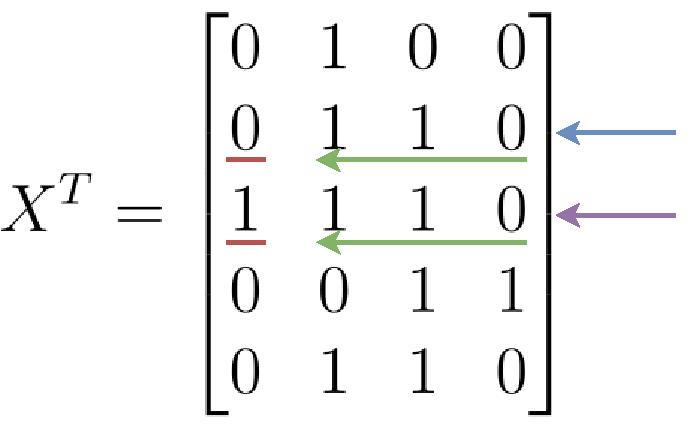
\includegraphics[scale = 0.38]{img/slppanel.pdf}
  \end{figure}
  Si procede quindi salvano la sequenza lineare relativa al pannelli come
  descritto sopra,
  ottenendo, con colorate gli stessi risultati della query fatta
  sopra:
  \[0010\,\,{\color{nordgreen}011}{\color{nordred}0}\,\,
    {\color{nordgreen}011}{\color{nordred}1} \,\,1100\,\,0110\]
  \textit{Si noti che qui si sono segnalate le varie righe con uno spazio ma
    solo per praticità ``visiva''.}
\end{esempio}
\textbf{ESEMPIO MAGARI DA SCRIVERE MEGLIO}
\subsubsection{LCE query}
Grazie all'uso delle \textit{LCE query} è quindi possibile calcolare l'array
delle \textit{matching statistics} in un solo scorrimento da sinistra a
destra. Infatti è possibile usare tali query per calcolare non solo quale nuova
sequenza scegliere in caso di mismatch con l'aplotipo query in colonna $i$, come
si faceva con l'uso delle \textit{threshold}, ma anche di computare la lunghezza
del suffisso comune tra essa e l'aplotipo query, calcolando nello stesso momento
sia $MS[i].row$ che $MS[i].len$.\\
Anche in questo caso, per convenzione, si inizia la computazione dell'ultima
riga della prima colonna.\\
Si illustra ora come computare l'array delle \textit{matching statistics}.
Si assuma di avere calcolato l'array $MS$ di una query $z$ rispetto al pannello
$X$. le cui righe si identificano tramite $x_i, \forall i\in\{0,M\}$, fino alla
colonna $k-1$. Sia $i$ 
l'indice di riga sulla \textit{matrice PBWT} al quale si è arrivati mediante il
mapping, avendo che tale riga è quella che ha il più lungo suffisso comune con
$z[1,k-1]$. Si assuma che l'indice $i$ appartenga alla run $r$, di simboli
$\sigma$, testa di indice $h$ e coda di indice $e-1$. Si hanno diversi casi:
\begin{enumerate}
  \item $z[k]=\sigma$, quindi la riga $i$ può essere usata per estendere il
  match, avendo che $MS[k].row=MS[k-1].row$ e $MS[k].len=MS[k-1].len+1$, e per
  proseguire col mapping in colonna $k+1$
  \item $z[k]\neq\sigma$ e si una sola run in colonna $k$, avendo quindi che non
  si possono avere match. Per convenzione, si
  imposta che $MS[k].row = M$ e $MS[k].len=0$. Infine si ricomincia, in colonna
  $k+1$, dall'ultima posizione, indicizzata nel pannello originale dal valore
  finale del \textit{prefix array sample} dell'ultima run
  \item $z[k]\neq\sigma$ ma si hanno anche altre run, dovendo quindi scegliere
  la nuova riga da seguire. Si ha che il più lungo suffisso di $z[1,k]$ che è
  anche suffisso di $x_1[1,k],\ldots, x_m[1,k]$ è uno tra:
  \begin{itemize}
    \item $x_{a_k[h-1]}$, se $h\neq 0$, ovvero la riga del pannello
    corrispondente alla fine della run precedente a $r$ nella \textit{matrice
      PBWT}, se esistente
    \item $x_{a_k[e+1]}$, se $e\neq M-1$, ovvero la riga del pannello
    corrispondente all'inizio della run successiva a $r$ nella \textit{matrice
      PBWT}, se esistente
  \end{itemize}
  Avendo quindi i \textit{prefix array sample} che ci dicono a quale riga nel
  pannello corrispondano tali valori e conoscendo $MS[k-1].row$ è possibile
  calcolare $LCE(MS[k-1].row, a_k[h-1])$ e $LCE(MS[k-1].row, a_k[e+1])$. A
  questo punto si sceglie il suffisso comune più lungo tra le due, ovvero il
  maggiore tra i valori ritornati dalla \textit{LCE query} e si sceglie la riga
  corrispondente per proseguire. Si ha quindi o $MS[k].row=a_k[h-1]$ o
  $MS[k].row=a_k[e+1]$. In merito alla lunghezza, assumendo che il miglior
  valore ritornato dalle due \textit{LCE query} sia $l$, si ha che:
  \[MS[k].len=\min(MS[k-1].len, l)+1\]
  In quanto la LCE query potrebbe restituire un valore più lungo dell'effettivo
  match con al query $z$ quindi si sceglie il minimo tra le due lunghezze,
  ottenendo l'effettiva lunghezza del suffisso comune tra $z$ e la nuova riga
  scelta fino a $k-1$, e lo si 
  incrementa di uno, contando il match ottenuto in colonna $k$
\end{enumerate}
\textbf{SISTEMARE}
\begin{esempio}
  Riprendiamo l'esempio \ref{es:thr}, visto per il calcolo
  tramite \textit{threshold}. \\
  Senza usare le \textit{threshold}, nella medesima situazione si dovrebbe
  calcolare, avendo che $MS[1].row=19$ e $MS[1].len =2$:
  \[LCE_1(x_{19}, x_{16})=2\]
  \[LCE_1(x_{19}, x_{17})=1\]
  Come verificabile dal pannello presente all'esempio \ref{es:pbwt1}.\\
  Si ha quindi che $MS[2].row=16$. Inoltre, sempre per quanto detto sopra:
  \[MS[2].len=\min(MS[1].len, 2)+1=2+1=3\]
\end{esempio}
Con questa variante quindi:
\begin{itemize}
  \item non si necessita di tenere in memoria le informazioni per le
  \textit{threshold}
  \item si tiene in memoria il pannello sotto forma di \textit{SLP}, soluzione
  vantaggiosa dal punto di vista della memoria anche se svantaggiosa da quello
  temporale (come descritto nella sezione \ref{slpsec})
  \item si permette il calcolo dell'array $MS$ in una singola scansione del
  pattern 
\end{itemize}
\textbf{Essendo lo scopo principale della tesi la riduzione dello spazio
  occupato dalla struttura dati questa è la soluzione migliore, avendo in
  memoria una struttura run-length encoded per la PBWT in grado di permettere
  pattern matching con un aplotipo esterno}.
